\chapter{Háttérinformációk}

\section{A \emph{syslog-ng}-ről}

\subsection{A fejlesztéshez használt technológiák}

Ebben az alszekcióban szeretném bemutatni azokat az eszközöket, amelyek a fejlesztéshez nap mint nap
használunk.

\begin{description}
    \item[JIRA] {Az Atlassian által fejlesztett, elsősorban hibajegyek kezelésére használatos
        szoftver. Esetünkben a \emph{VersionOne}-t váltotta le.}
    \item[ZBS] {asd }
    \item[ZTS] {asd }
    \item[git] {A git már egy nagy múltra visszatekintő (először 2005-ben adták ki), eredetileg a
        Linux kernel fejlesztését segítő, elosztott verziókezelő rendszer. Elosztottságának
        köszönhetően a nyílt forráskódú szoftverek világában az egyik legnagyobb mértékben
        adoptált, köztük a \emph{syslog-ng} fejlesztésénél is ezt használjuk mindkét változatában.
        (Kereskedelmi termékek fejlesztésénél ez annyira nem jellemző, nekünk viszont erősen
    ajánlott azért, hogy a két változat közötti kódmozgatás gördülékenyebb legyen.)}
    \item[GitHub] {Habár egy egyszerű tárhelynek tűnhet csupán, mégis az általa adott
        többletszolgáltatások a közösség által fejlesztett syslog-ng központi elemévé tette.
        Ilyen többletszolgáltatás a \emph{forkok} könnyű kezelése, a beépített hibajegykezelő,
        a \emph{pull request}-ek könnyű kezelése (azaz a GitHub-on lévő forkomból pár
        kattintással tudok kontribúciót küldeni az \emph{upstream repository}-ba), és a könnyű
        bővíthetősége, például lektorálást segítő eszközökkel, \emph{Continous Integration}-t
        megvalósító eszközökkel, statikus kódanalízist biztosító eszközökkel.
        Természetesen a névválasztás nem véletlen, nagyban épít a korábban említett \emph{git}
        verziókezelőre.}
\end{description}

\subsection{A fejlesztés során felmerülő problémák}

A teljesség igénye nélkül listázzuk a fejlesztést nehezítő, olykor értékes fejlesztői időt pazarló
problémákat:
\begin{itemize}
    \item Lassú lektorálási folyamat a közösség által fejlesztett változatban:
\end{itemize}

Ennek egy részproblémája az, hogy
\begin{itemize}
    \item a kód automatikusan formázva.
\end{itemize}
Érdekesség, hogy a \emph{CVE-2014-1266}, közismertebb nevén \emph{goto fail;} sérülékenységet egy
egyszerű \emph{code beautifier} figyelemfelkeltőbbé tette volna azáltal, hogy a tabulálásokat
(pontosabban fogalmazva \emph{indent}álásokat) helyessé tette volna.


\begin{itemize}
    \item Meredek tanulási görbe a belső eszközök használatánál:
\end{itemize}
, amelyből következik, hogy
\begin{itemize}
    \item a saját eszközök belső működéséhez kevesen értenek.
\end{itemize}
Ezért ennek a területnek definíció szerint alacsony a \emph{busz faktora}, amely hosszabb távon
nézve kockázatos mind biztonsági (szélsőséges esetben egy ember ismer egy rendszert igazán, így az
ő módosításainak lektorálása nem hatékony), mind 

\begin{itemize}
    \item Törékeny fejlesztési infrastuktúra.
\end{itemize}
Ez leginkább abban mutatkozik meg, hogy vannak olyan fejlesztői gépek, amelyeknél azok létrehozási
lépései elvesztek, illetve az idők során az azon végzett módosítások nem lettek megfelelően
dokumentálva. Amennyiben ez a fejlesztés szempontjából egy kritikus gép, belátható, hogy az egy
időzített bombaként viselkedik a rendszerben. Ennek a problémának egy tipikus áthidalása, ha az
adott gépről létezik visszaállítható biztonsági mentés, hiszen ekkor egy jól működő állapotra
visszaállhatunk, de az esetleges korszerűsítés (például frissebb operációs rendszerre való átállás)
még problémákat jelenthet.

Úgy gondoljuk, hogy ezek kijavítása ugyan kezdetben sok erőforrást igényelhetnek, de a későbbiekben
olyan mértékben egyszerűsítik a fejlesztők életét, hogy ez a befektetés megtérül.

Időközben magasabb vezetési szintről felmerült az igény, hogy legyünk tisztában a termékeink
\todo[inline]{Reword: }biztonsági állapotával, ezért mindenképpen kívánatos, ha a választott módszer
széleskörűen alkalmazható.

\section{Különböző megközelítések vizsgálata}

Az egyes megközelítések feltérképezéséhez és megvizsgálásához remek kiindulási alapot adott az
alábbi publikáció:
\url{http://citeseerx.ist.psu.edu/viewdoc/download?doi=10.1.1.132.4843&rep=rep1&type=pdf}.

\subsection{Attack trees}

Az \emph{Attack trees} egy olyan módszer, amellyel egy adott támadást elemezhetünk egyszerűen, egy
faként reprezentálva az alábbi szabályok mentén:
\begin{enumerate}
    \item A fa gyökerében az az esemény áll, amely bekövetkezésekor a támadást sikeresnek tekintjük.
    \item A szülő és a gyerek eseménye között az a kapcsolat, hogy a szülő eseménye akkor, és csak
        akkor következik be, ha a gyerek eseménye is.  Összekapcsolt gyerekek esetén akkor és csak
        akkor, ha mindegyik gyerek eseménye bekövetkezett.
\end{enumerate}
Miután megtaláltuk az eseményeink függőségeit (pontosabban a további felbontásnak már nem lenne
értelme), lehetőségünk van ezeket különféle szempontokból elemezni, például az alábbi szempontok
mentén:
\begin{itemize}
    \item Lehetséges-e egyáltalán az esemény bekövetkezése?
    \item Mekkora költséggel jár előidézni az eseményt?
    \item Mekkora költséggel jár megelőzni az eseményt?
    \item Szükséges-e különleges felszerelés az előidézéshez?
\end{itemize}

\missingfigure{Példa}

Az alábbi szempontok segíthetnek eldönteni, hogy megéri-e foglalkozni a védelem kialakításával,
szem előtt tartva, hogy mit feltételezünk a támadóról.

Habár a módszer kellően könnyedén értelmezhető (hiszen csupán egy fát használ) és könnyedén
alkalmazható, számunkra kevésbé használható, hiszen nem kellően széleskörű, és megoldásokat
egyáltalán nem szolgáltat, és a teljesség sem garantált.

\subsection{Abuse/Misuse cases}

Az \emph{Misuse cases} az ismert \emph{use case} diagramnak a kifordított változata, azaz ahelyett,
hogy azt modelleznénk, hogy egy adott szereplő milyen tevékenységeket végezhet el, itt inkább azt
modellezzük, hogy egy rosszindulatú szereplő milyen tevékenységeket végezne el, azaz
meghatározhatjuk azokat a tevékenységeket, amelyeket a \emph{rendszernek tiltania kellene}.

\begin{figure}[h]
    \centering
    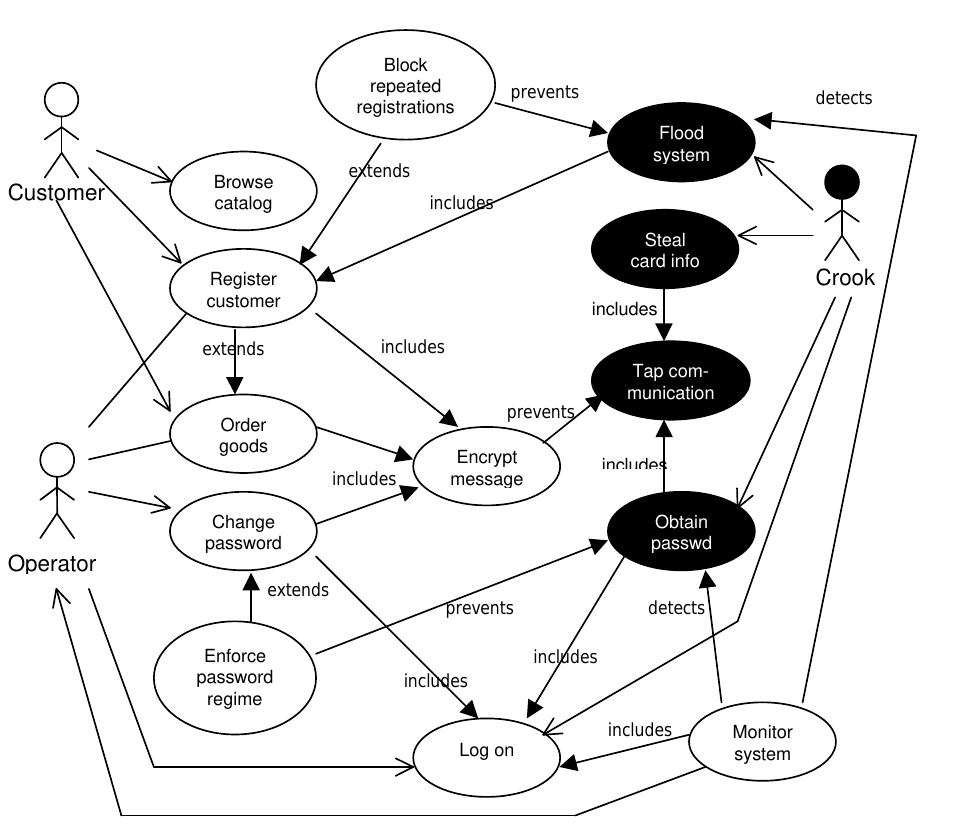
\includegraphics[width=\textwidth, height=0.5\textheight, keepaspectratio]{figures/misusecase.png}
\end{figure}

\FloatBarrier
\subsection{ISO 27000-as család}
\subsubsection{ISO 27001:2013}
Ellentétben a korábbi megközelítésekkel, az \emph{ISO 27001}-es szabvány 

Habár elsőre nem tűnik indokoltnak a megemlítése, elég csupán arra gondolnunk, hogy egy termék
fejlesztésekor elvárhatjuk, hogy a belső infrastruktúránk biztonságos.  Ahogy a cég (és ezzel együtt
az infrastruktúra) növekszik, egyre inkább fontossá válik egy olyan kész keret bevezetése, amelyet
felhasználva biztonságosabb rendszert építhetünk.

\subsection{Common Criteria}

\section{Miért választottuk a Common Criteria-t}

Végeredményként az alábbi metodologiákat kezdtük el alkalmazni:
\begin{itemize}
\item Common Criteria-t a 
\item{ISO 27001:2013-at az infrastruktúra (beleértve a számunkra releváns fejlesztői infrastruktúra)
    biztonságának erősítésére.}
\end{itemize}

A fő okok az alábbiak voltak:

\todo[inline]{Okok listázása}

\section{Common Criteria-ról bővebben}

\subsection{Terminológia}

A későbbiekben előforduló rövidítések itt kerülnek feloldásra.

\begin{description}
    \item[TOE]{Target of Evaluation - az az entitás, amelyre a \emph{Common Criteria} által
            megfogalmazott követelmények teljesülését vizsgáljuk. Esetünkben ez a \emph{syslog-ng}-re,
        mint szoftvercsomagra vonatkozik.}
    \item[EAL]{Evaluation Assurance Level - a követelmények szigorúságának számszerűsített értéke,
        lásd később.}
\end{description}

\subsection{Evaluation Assurance Levels}

Az \emph{Evaluation Assurance Level} (továbbiakban: EAL) egy egytől hétig tartó skálán egyre nagyobb
nyújt, pontosabban a magasabb szinteknél szigorúbb elvárásoknak kell megfelelni. A szigorúbb
elvárásoknak való megfelelőség óhatatlanul magasabb költségekkel is járhat, így az elérni kívánt
szint meghatározásánál figyelembe kell venni, hogy milyen előnyökkel és költségekkel jár annak
elérése. \cite{DipPortal}

\subsubsection{EAL1: funkcionálisan tesztelt}
\todo[inline]{Célja}
\todo[inline]{Miben több, mint az EAL0?}

\subsubsection{EAL2: strukturálisan tesztelt}
\todo[inline]{Célja}
\todo[inline]{Miben több, mint az EAL1?}

\subsubsection{EAL3: metodilikusan tesztelt és ellenőrzött}
\todo[inline]{Célja}
\todo[inline]{Miben több, mint az EAL2?}
\subsubsection{EAL4: }
\todo[inline]{Célja}
\todo[inline]{Miben több, mint az EAL3?}
\subsubsection{EAL5:}
\todo[inline]{Célja}
\todo[inline]{Miben több, mint az EAL4?}
\subsubsection{EAL6:}
\todo[inline]{Célja}
\todo[inline]{Miben több, mint az EAL5?}
\subsubsection{EAL7:}
\todo[inline]{Célja}
\todo[inline]{Miben több, mint az EAL6?}
